\chapter{Meltdown e il sistema di protezione KAISER}
\label{cap:meltdown}
La sicurezza dei sistemi informatici attuali si fonda sull'isolamento della memoria,
ad esempio marcando come privilegiati gli indirizzi di memoria kernel e bloccando eventuali
accessi da parte di programmi utente \cite{lettieri:protezione}. 
\textbf{Meltdown} è un tipo di attacco informatico che sfrutta un effetto
collaterale dell'esecuzione fuori ordine nei processori moderni per leggere locazioni di memoria scelte in maniera
arbitraria. L'attacco funziona su varie microarchitetture Intel prodotte sin dal 2010, indipendentemente dal sistema
operativo in uso. Meltdown è quindi in grado di accedere arbitrariamente a qualsiasi locazione di memoria protetta
(afferenti al kernel o ad altri processi) senza necessitare alcun permesso o privilegio da parte del
sistema \cite{lipp:meltdown}.

Meltdown rompe quindi tutti i meccanismi di sicurezza che si basano sull'isolamento degli spazi di indirizzamento, andando a colpire milioni di utenti. Il sistema di protezione KAISER, sviluppato originariamente per KASLR \cite{gruss:kaslr}, ha l'importante effetto secondario di impedire l'utilizzo di Meltdown \cite{lipp:meltdown}.

L'obiettivo di questa tesi è stato quello di proteggere da Meltdown il nucleo didattico utilizzato nel corso di "Calcolatori Elettronici" tenuto dall'Ing. Giuseppe Lettieri, implementando una versione ottimizzata di KAISER.

Nella nostra trattazione, mostreremo prima le caratteristiche e le cause dell'attacco Meltdown e in che modo il sistema KAISER possa proteggere il kernel da questo tipo di attacco (capitolo \ref{cap:meltdown}).
Dopodiché verranno descritte le caratteristiche peculiari del nucleo didattico (capitolo \vref{cap:nucleo}). 
Infine, concluderemo con la presentazione delle modifiche apportate al nucleo (capitolo \vref{cap:implementazione}) e con il codice prodotto (capitolo \vref{cap:codice}).


\section{Background}
Presenteremo ora sinteticamente tre concetti alla base dell'attacco Meltdown: l'esecuzione fuori ordine, gli spazi di indirizzamento e gli attacchi alla memoria cache.

\subsection{Esecuzione Fuori Ordine}
\label{sec:esecuzione-fuori-ordine}
L'esecuzione fuori ordine è una tecnica di ottimizzazione che permette di massimizzare l'utilizzo delle unità di esecuzione della CPU~\cite{lipp:meltdown}.
Ogni istruzione Assembly viene prelevata dalla memoria e poi decodificata dalla CPU, ovvero viene tradotta in una o più \emph{micro-operazioni}.
La CPU non segue il flusso lineare di istruzioni, ma esegue ogni micro-operazione \emph{non appena tutte le risorse necessarie sono disponibili} (che siano risorse hardware o dati restituiti da altre operazioni).
Si dice quindi che la CPU non esegue le istruzioni linearmente, ma \textbf{in maniera speculativa}~\cite{frosini:calcolatori2}.

Le micro-operazioni vengono inserite in una coda di riordino nell'ordine previsto dal programma.
Gli effetti di una micro-operazione completata senza errori possono essere applicati sulla RAM e sui registri visibili quando non vi sono altre micro-operazioni davanti nella coda.
Si dice, in questo caso, che la micro-operazione (o in senso più largo, l'istruzione) viene \emph{ritirata}~\cite{frosini:calcolatori2}.
Si noti che le istruzioni vengono ritirate dalla CPU nell'ordine in cui sarebbero state eseguite se la CPU avesse seguito in maniera lineare il flusso d'istruzioni.

Nell'esecuzione fuori ordine, è comune che vengano eseguite (ma non ritirate) alcune istruzioni che non fanno parte del flusso lineare di controllo~\cite{frosini:calcolatori2}, dette \emph{transient instruction}~\cite{lipp:meltdown}.
Questo è dovuto al fatto che la CPU cerca di "indovinare" la direzione che intraprende il flusso di istruzioni in corrispondenza di una istruzione di salto, sfruttando tecniche predittive che variano a seconda dell'hardware~\cite{frosini:calcolatori2}.

Nel caso di una predizione di salto \emph{errata}, le istruzioni \emph{non} vengono ritirate e gli effetti vengono annullati (\emph{rollback delle istruzioni}).
In questo modo, le transient instruction non hanno alcun effetto sulla macroarchitettura (memoria centrale e registri visibili del processore).

\subsection{Spazi di indirizzamento}
\label{sec:spazi-di-indirizzamento}
\begin{figure}
	\centering
	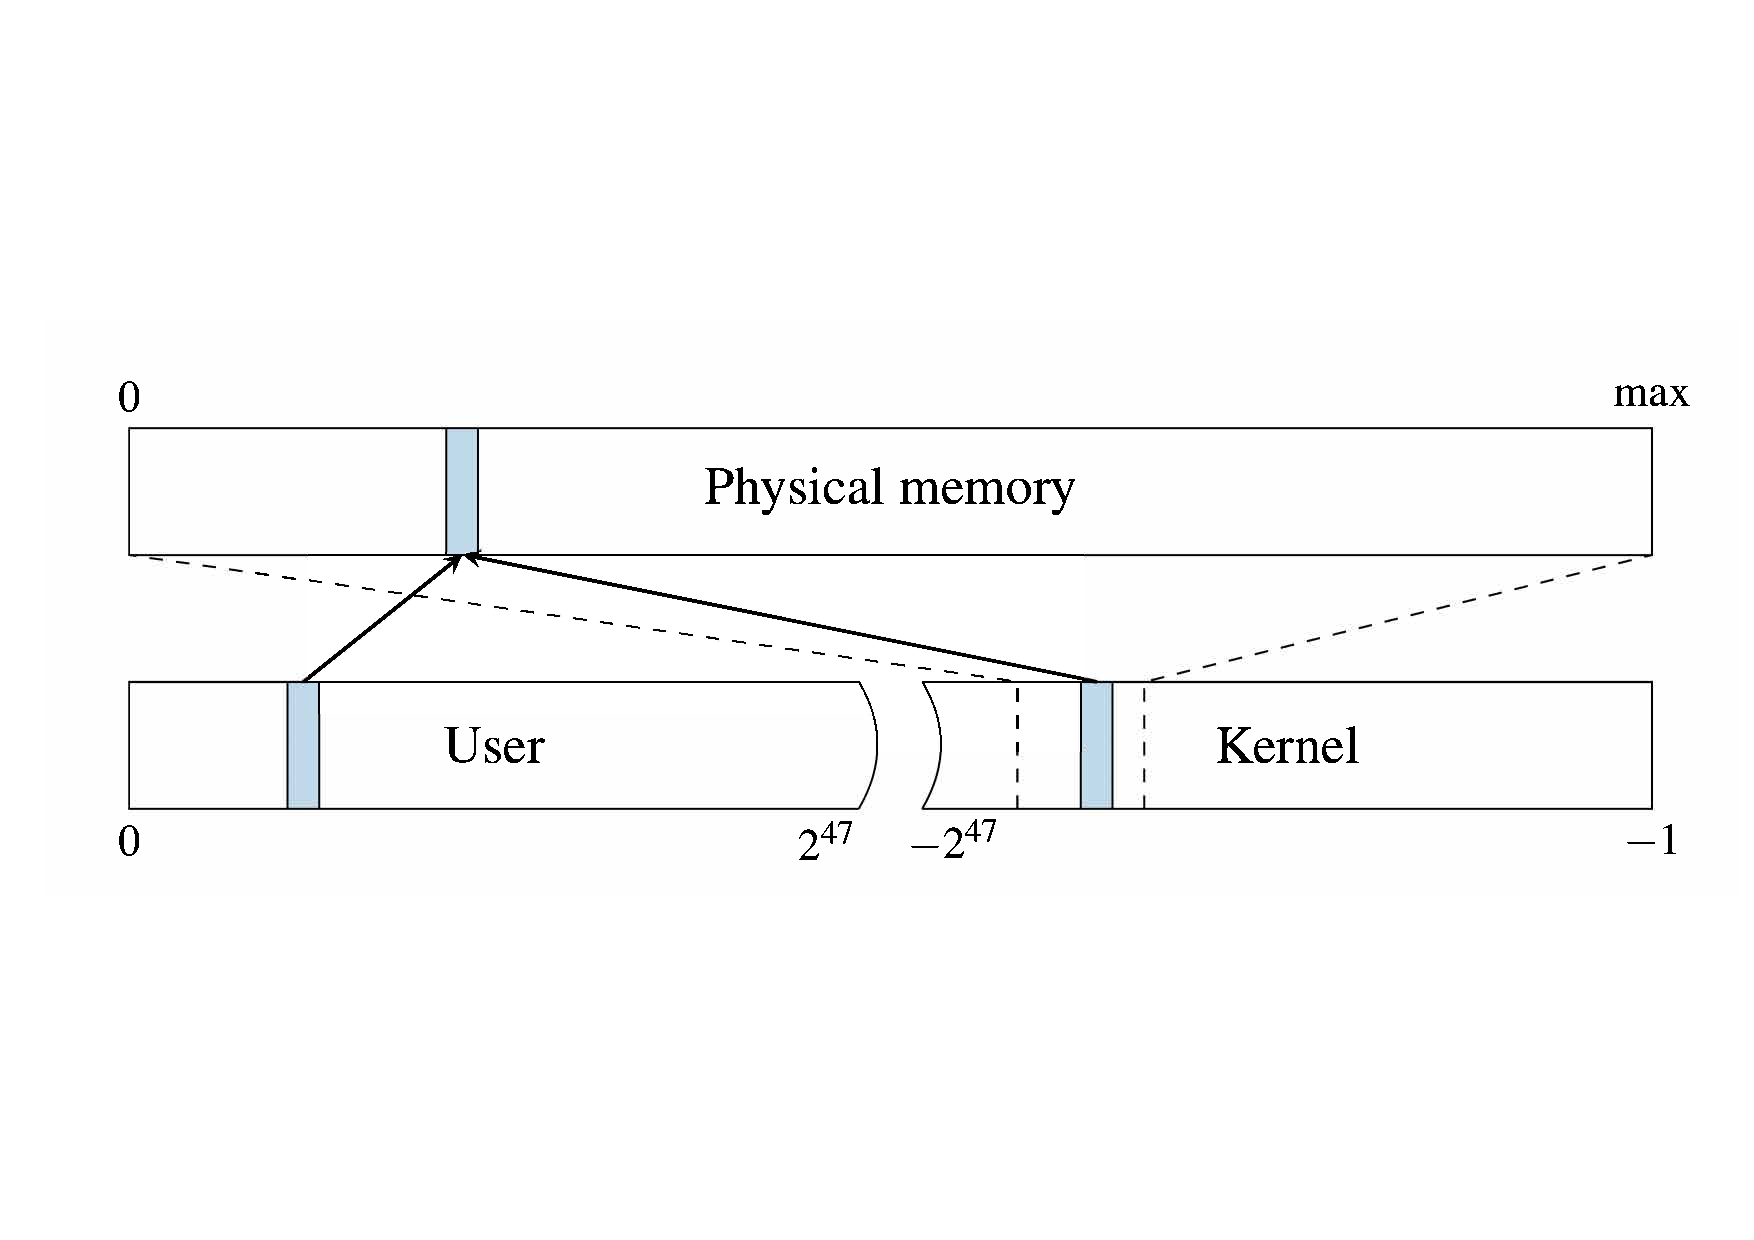
\includegraphics[width=0.7\textwidth]{"img/memoria-fisica.pdf"}
	\caption{Ogni indirizzo fisico del processo è mappato sia nello spazio d'indirizzamento utente che in quello kernel all'interno della finestra di memoria fisica}
	\label{fig:memoria-fisica}
\end{figure}

Per risolvere diversi problemi, in particolare l'isolamento dei processi \cite{lettieri:paginazione}, le CPU supportano l'utilizzo di spazi d'indirizzamento virtuali, in cui gli indirizzi virtuali (relativi al singolo processo) vengono tradotti in indirizzi fisici. 
Lo spazio d'indirizzamento di un processo (ovvero tutti i possibili indirizzi che un processo può generare) viene suddiviso in regioni dette \emph{pagine} che possono essere mappate individualmente nella memoria fisica attraverso una tabella di traduzione multivello. 
Ogni processo possiede una propria tabella di traduzione che traduce tutti e soli i suoi indirizzi virtuali e che definisce le proprietà di protezione delle varie zone di memoria. 

Per permettere ad ogni processo di usufruire delle primitive di sistema offerte dal kernel e alle routine di sistema di accedere liberamente all'intera memoria fisica (ad esempio per modificare le tabelle di traduzione di un processo), si utilizza una traduzione, denominata \emph{finestra di memoria fisica}, che mappi l'intera memoria fisica, compresi il kernel e lo spazio di memoria di tutti i processi, nello spazio di indirizzamento accessibile solo da livello privilegiato (figura \vref{fig:memoria-fisica})~\cite{lettieri:paginazione-complementi}.


\subsection{Attacchi Cache}
Al fine di velocizzare gli accessi alla RAM, le CPU contengono buffer di memoria molto veloce ma di dimensioni limitate che costituiscono la cosiddetta \emph{memoria cache}. La memoria cache maschera i tempi di latenza estremamente lunghi per l'accesso alla memoria centrale (molto lenta in confronto alla cache) conservando le locazioni di memoria che, secondo principi statistici come la \emph{località spaziale} (se un programma accede ad un certo indirizzo, è molto probabile che in breve tempo accederà ad un indirizzo vicino)  e la \emph{località temporale} (se un programma accede ad un certo indirizzo, è molto probabile che in breve tempo vi accederà di nuovo), è più probabile vengano indirizzate dalla CPU nel breve periodo \cite{lettieri:cache}.

Gli attacchi a canale laterale (\emph{side-channel attacks}) contro la cache sfruttano questa differenza di tempo di accesso introdotta dalla cache stessa. Negli attacchi Flush+Reload \cite{yaron:flush-reload}, usati da Meltdown \cite{lipp:meltdown}, l'attaccante è in grado di determinare se una locazione di memoria è stata precedentemente caricata in cache, misurando il tempo impiegato da un'operazione di lettura.

%%
\section{Come agisce Meltdown}
L'attacco Meltdown consiste in tre passi fondamentali \cite{lipp:meltdown}:
\begin{enumerate}
	\item Leggere il contenuto di una locazione di memoria inaccessibile dall'attaccante, causando il lancio di un'eccezione di protezione
	\item Accedere in maniera speculativa ad una linea di memoria cache in base al contenuto segreto della locazione protetta
	\item Usare un'attacco di tipo Flush+Reload per determinare il contenuto segreto in base a quale linea di memoria è stata acceduta
\end{enumerate}

\subsection{Passo 1: Leggere il segreto}
Nel prima passo di Meltdown, l'attaccante cerca di accedere ad una zona di memoria protetta, ad esempio la memoria kernel.
Il tentativo di accesso ad una pagina non accessibile da livello utente fa in modo che la CPU sollevi un'eccezione di protezione, che generalmente termina il processo. 
Tuttavia, a causa dell'esecuzione fuori ordine, la CPU potrebbe aver già eseguito l'istruzione di accesso in maniera speculativa \emph{prima} delle istruzioni relative all'eccezione di protezione, al fine di minimizzare i tempi di latenza (vedi paragrafo \ref{sec:esecuzione-fuori-ordine}).
In questo modo la CPU accederebbe in maniera speculativa alla locazione di memoria desiderata prima che il processo venga terminato.

Grazie al lancio dell'eccezione, le eventuali istruzioni eseguite in maniera speculativa, che non sarebbero docute essere eseguite in quanto relative ad una previsione di salto \emph{errata}, non vengono \emph{ritirate} dalla CPU e non hanno così alcun effetto sulla macroarchitettura in generale (memoria centrale e registri logici non speculativi del processore) \cite{frosini:calcolatori2}.

\subsection{Passo 2: Trasmettere il segreto}
\label{sec:meltdown-passo-2}
Per poter trasmettere il segreto, si utilizza un \emph{probe array}, di dimensione pari a 256 pagine virtuali e allocato precedentemente nella memoria del processo attaccante, assicurandosi che \emph{nessuna porzione dell'array sia presente nella cache}. 
La sequenza di transient instruction contiene un accesso ad un elemento del probe array, il cui offset è calcolato moltiplicando il valore del byte per la dimensione di una pagina virtuale (tipicamente e nel nostro sistema  è \emph{4KiB}~\cite{lettieri:paginazione}).

Quando la CPU gestisce l'eccezione di protezione causata dal Meltdown, le transient instruction non vengono ritirate dalla CPU, senza avere dunque effetti a livello di macroarchitettura. Sebbene quindi non sia possibile rendere direttamente disponibile il segreto dal programma utente, si hanno importanti effetti secondari a livello di microarchitettura, in particolare nella memoria cache~\cite{lipp:meltdown}.

Durante l'esecuzione speculativa, infatti, la locazione di memoria all'interno del probe array che viene acceduta dalla CPU, viene memorizzata in memoria cache e vi rimane anche in seguito all'annullamento degli effetti delle transient instruction, rendendola vulnerabile ad un attacco side-channel.

L'utilizzo del valore segreto moltiplicato per la dimensione della pagina, ci garantisce sia una precisa \emph{correlazione} tra il valore segreto e la locazione caricata in memoria, sia che a differenti valori della locazione di memoria saranno accedute differenti \emph{pagine} del probe array.
Ciò previene il fatto che il prefetcher hardware (per ragioni di ottimizzazione) potrebbe caricare in cache anche le locazioni di memoria adiacenti a quella acceduta, rendendo impossibile determinare quale locazione di memoria sarebbe stata indirizzata se non fosse stato utilizzato a priori questo accorgimento.

\subsection{Passo 3: Ricevere il segreto}
\label{sec:meltdown-passo-3}

\begin{figure}
	\centering
	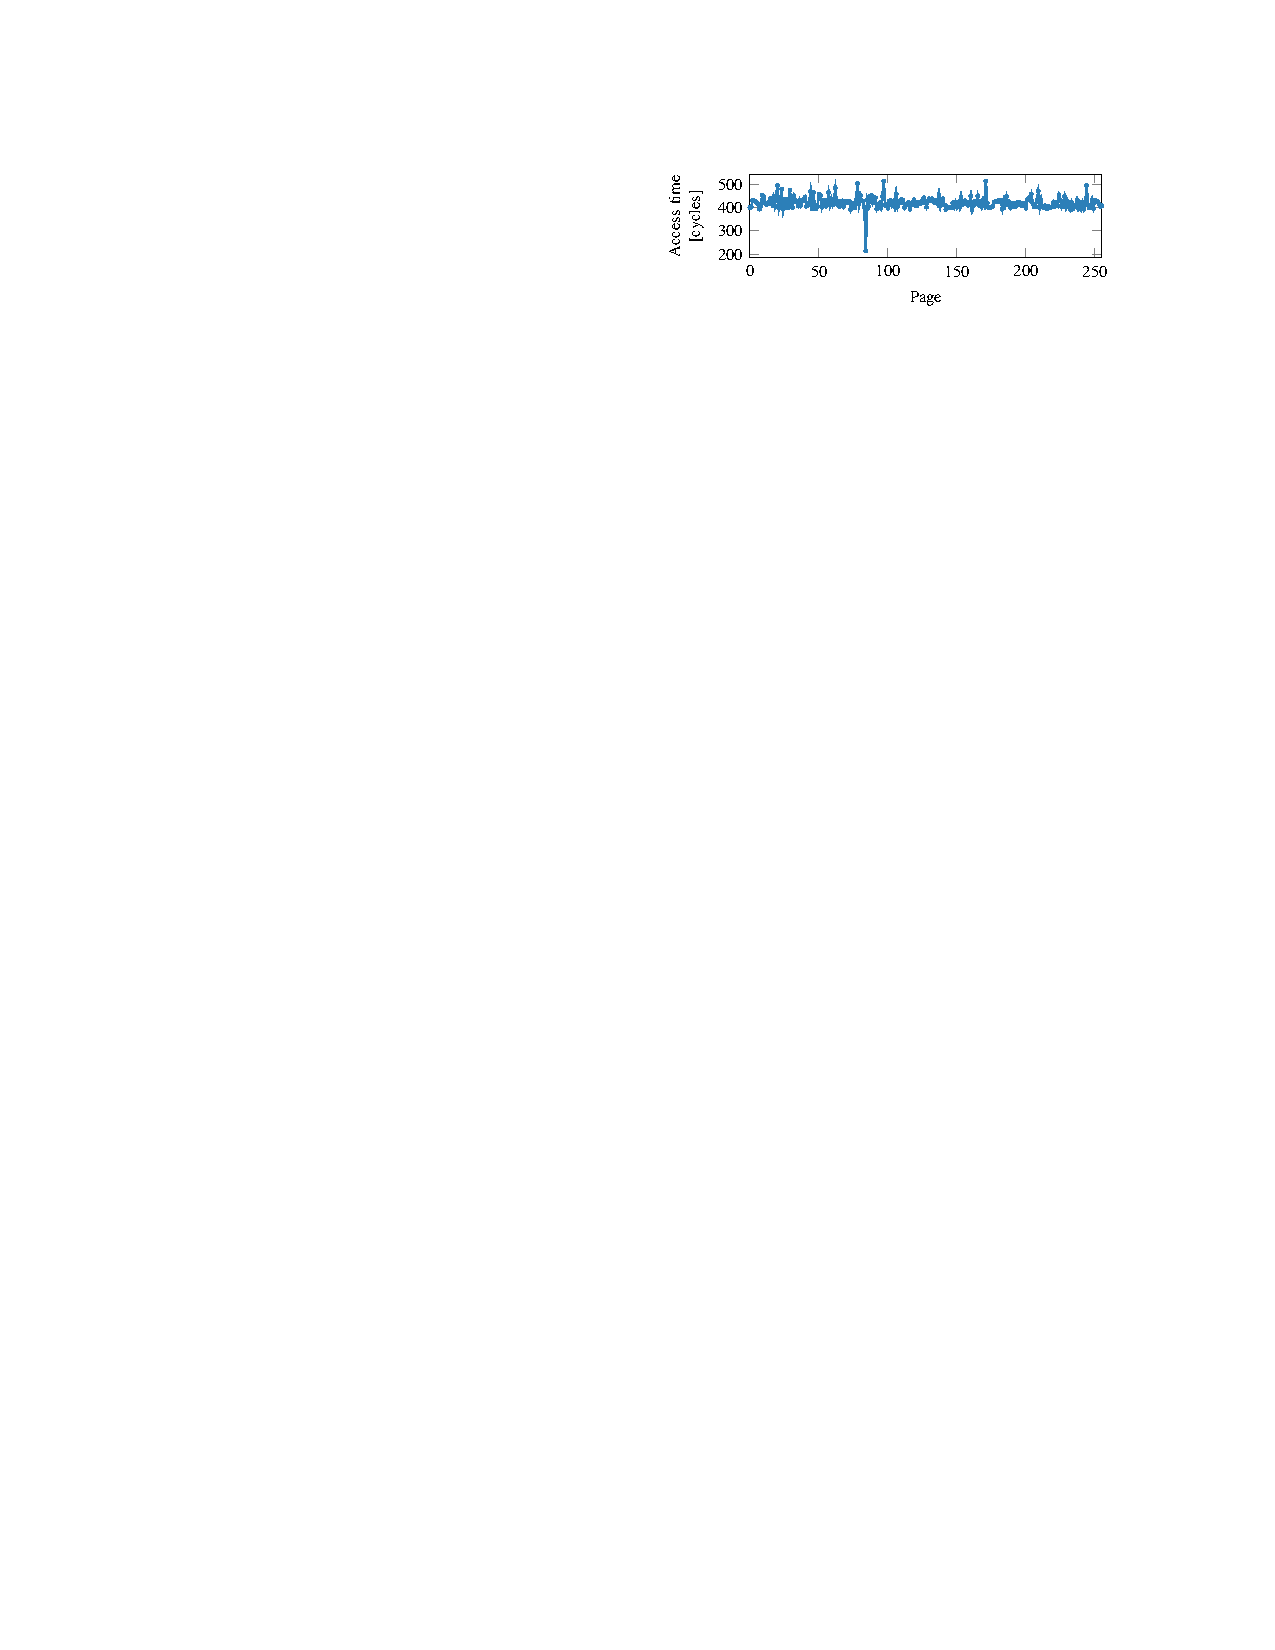
\includegraphics[width=0.75\textwidth]{"img/probe-array.pdf"}
	\caption{Tempo di accesso alle 256 pagine del probe array. Il grafico mostra una \emph{cache hit} sulla pagina acceduta nel passo~2.~\cite{lipp:meltdown}}
	\label{fig:probe-array}
\end{figure}

Dopo che la sequenza di istruzioni del passo 2 è stata eseguita, in cache è presente esattamente una linea di memoria del probe array.
L'offset di questa linea è dipendente esclusivamente dal valore segreto presente nell'arbitaria locazione di memoria protetta.
Grazie a ciò, l'attaccante può effettuare un'attacco Flush+Reload~\cite{yaron:flush-reload}, iterando attraverso le 256 pagine del probe array e misurando il tempo di accesso per il primo elemento di ogni pagina (vedi figura \ref{fig:probe-array}).
In base a quanto detto finora, la pagina con la latenza minore è l'unica presente in memoria cache e il numero della pagina è il valore segreto letto dalla memoria protetta.


\subsection{Conclusioni}
\label{sec:meltdown-conclusioni}
Il seguente codice mostra in Assembly x86-64 la sequenza di istruzioni alla base di Meltdown, relative ai passi 1 e 2 dell'attacco.

\begin{lstlisting}[
	language={[x64]Assembler},
	frame=single,
	numbers=left, numbersep=7pt,
	xleftmargin=18.5pt,
	xrightmargin=-18.5pt,
	framexleftmargin=13pt,
	framexrightmargin=-20.5pt,
	basicstyle=\ttfamily\onehalfspacing,
	keywordstyle=\bf
	]
# rcx = indirizzo di memoria kernel
# rbx = probe array
movb (%rcx), %al         # Lettura del segreto
shl  $12, %rax           # Traslazione dell'offset
movq (%rbx, %rax), %rbx  # Trasmissione del segreto
\end{lstlisting} 

Meltdown è quindi in grado di leggere in maniera arbitraria dati presenti in memoria \emph{protetta}, ad esempio nello spazio di indirizzamento kernel. 
L'efficienza di Meltdown si basa principalmente sull'esistente \emph{race condition} tra il lancio dell'eccezione di protezione e il passo 2 del nostro attacco (vedi paragrafo \vref{sec:meltdown-passo-2}). Per questo motivo, sono previsti alcuni accorgimenti e ottimizzazioni ulteriori non significativi per la nostra trattazione e per le quali rimandiamo a \textcite{lipp:meltdown}.

Dato che l'intera memoria fisica viene mappata all'interno dello spazio di indirizzamento del kernel attraverso la cosiddetta \emph{finestra di memoria fisica}~\cite{lettieri:paginazione-complementi}, Meltdown è in grado non solo di leggere le zone di memoria relative al kernel, ma anche gli spazi di memoria di tutti gli altri processi. In base a quanto rilevato da \textcite{lipp:meltdown}, Meltdown è in grado di effettuare il dump dell'intera memoria fisica fino ad una velocità di 503 KB/s.

%%
\section{Il sistema di protezione KAISER}
\label{sec:kaiser}
KAISER, proposto da \textcite{gruss:kaslr}, è una modifica del nucleo in cui il kernel non viene mappato nello spazio virtuale dei processi utente.
Questa modifica era stata pensata per prevenire attacchi side-channel contro la misura di protezione KASLR \cite{hund:practical-timing-side-channel, gruss:prefetch-side-channel-attacks, jang:breaking-kaslr}, ma ha l'importante effetto secondario di prevenire Meltdown~\cite{lipp:meltdown}.

L'idea alla base di KAISER è quella di separare lo spazio di memoria kernel da quello utente, ovvero di rendere disponibile la traduzione degli indirizzi virtuali del kernel \emph{soltanto} quando il sistema si trova in modalità privilegiata.
Ciò previene Meltdown in quanto, quando il sistema sta eseguendo il programma utente della sezione \vref{sec:meltdown-conclusioni}, l'indirizzo virtuale scelto non è presente nell'albero di traduzione del processo attaccante e quindi la CPU non è in grado di accedervi neanche in maniera speculativa.
Il meccanismo proposto da \citeauthor{gruss:kaslr} è quindi ritenuto la miglior soluzione a breve termine per proteggere i sistemi informatici da Meldown~\cite{lipp:meltdown}.

KAISER introduce il concetto di \textbf{spazi d'indirizzamento shadow} per garantire l'isolamento della memoria kernel. 
Come mostrato in figura \vref{fig:memoria-shadow}, ogni processo possiede due spazi di indirizzi: uno spazio d'indirizzamento shadow, in cui è mappato solo lo spazio di memoria utente e una porzione del kernel necessaria per le interruzioni, e uno spazio d'indirizzamento in cui è mappato sia l'intero kernel che lo spazio utente, protetto con Supervisor Mode Access Prevention (SMAP) e Supervisor Mode Execution Prevention (SMEP) per combatibilità con x86 Linux~\cite{gruss:kaslr}.

Ogni qualvolta che il programma passerà da livello utente a livello sistema (ad esempio attraverso una primitiva di sistema o il lancio di un'interruzione) e viceversa, la CPU dovrà aggiornare il registro CR3 con il valore della tabella di livello 4 corrispondente al nuovo livello di privilegio (tabella shadow per il livello utente e tabella kernel per il livello sistema). 
Sarà dunque necessario implementare una o più funzioni (le \emph{funzioni trampolino}), mappate in memoria shadow, dedicate all'aggiornamento corretto del registro CR3 ad ogni modifica del livello di privilegio.

\begin{figure}
	\centering
	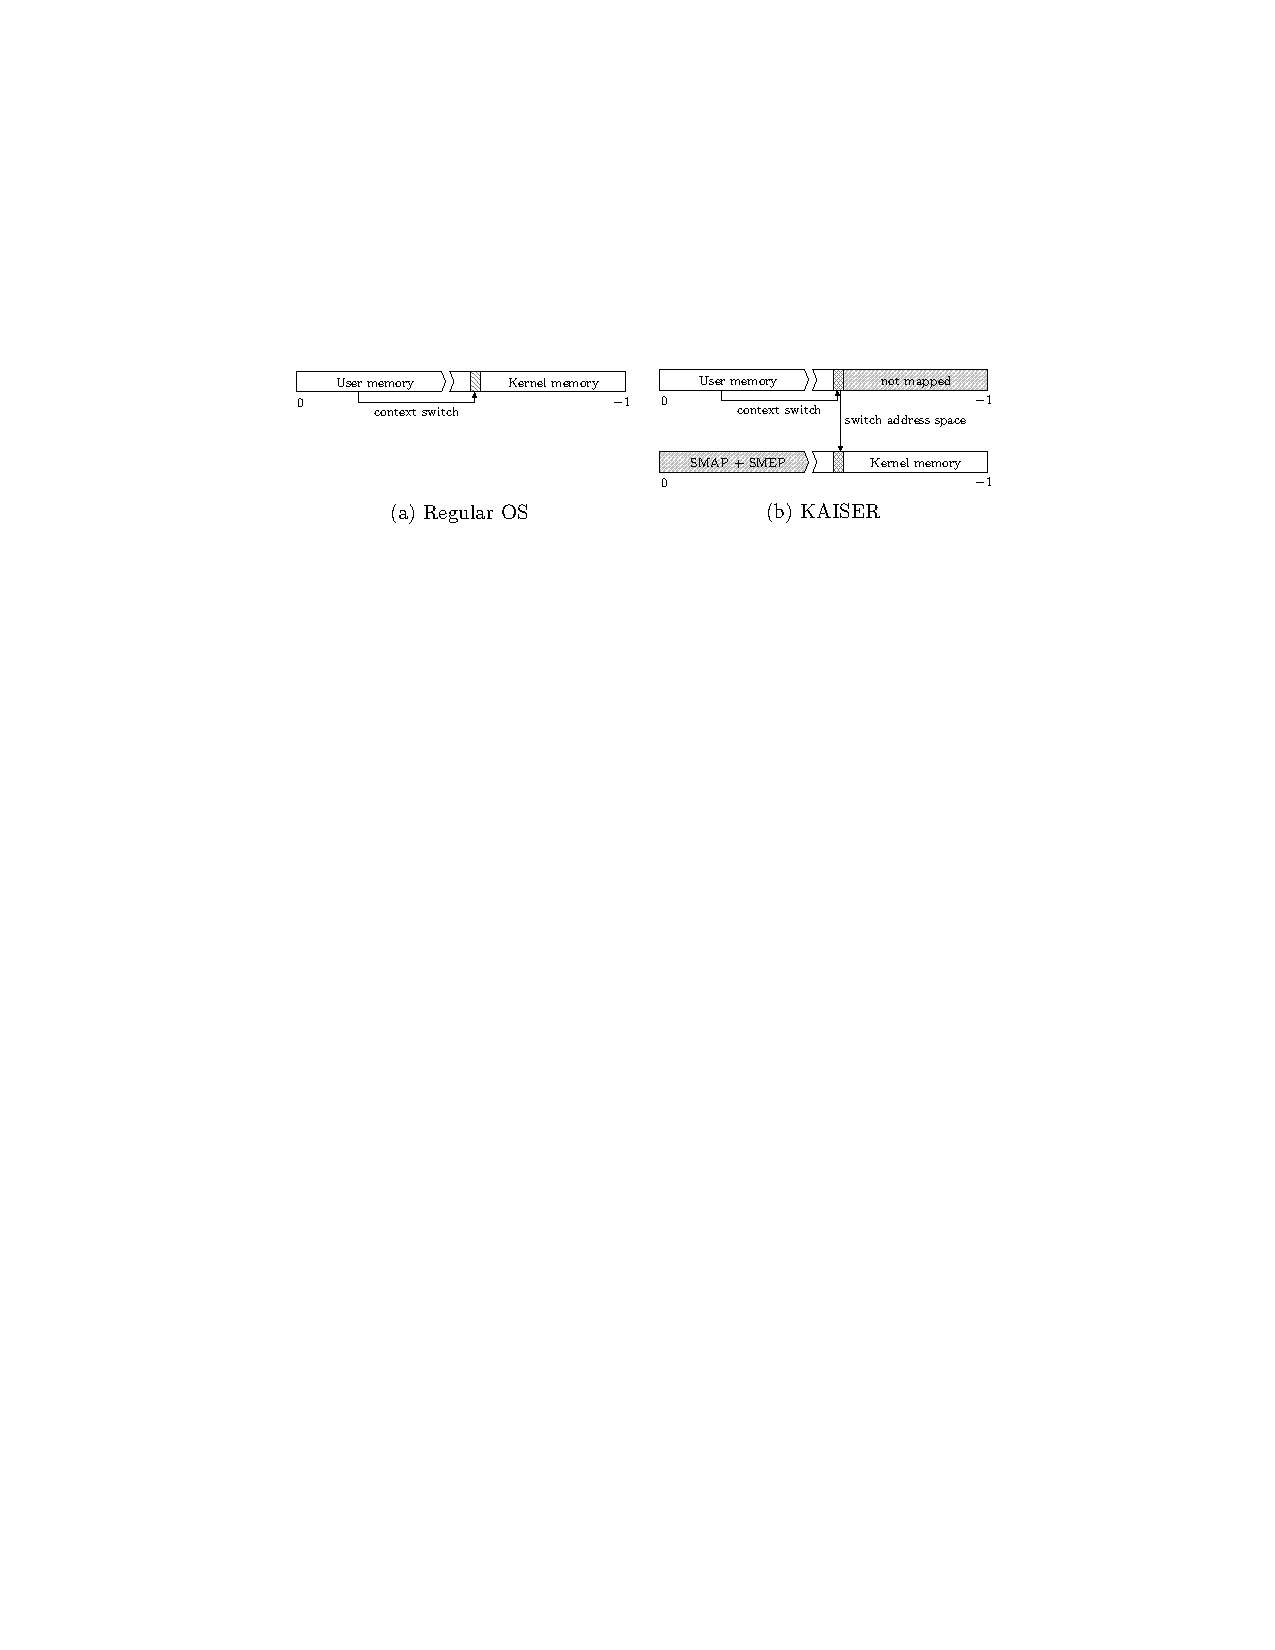
\includegraphics[width=\textwidth]{"img/memoria-shadow.pdf"}
	\caption{(a) Il kernel è mappato nella memoria virtuale di ogni processo. (b) TODO}
	\label{fig:memoria-shadow}
\end{figure}

Come accennato sopra, nell'architettura x86 sono necessarie alcune porzioni del kernel per il corretto funzionamento delle interruzioni e devono perciò essere mappate nello spazio di indirizzamento shadow:
\begin{itemize}
	\item la Interrupt Descriptor Table (IDT);
	\item la Global Descriptor Table (GDT);
	\item i Task State Segment (TSS);
	\item la pila sistema del processo;
	\item la pila e il vettore delle richieste di interruzioni;
	\item il codice di entrata e uscita dagli interrupt handler.
\end{itemize}
